The CORDET Framework is an application-level framework and its domain is the management of services. Service messages encapsulating commands and reports are exchanged between applications. The mechanism through which these messages are sent from one application to another is outside the scope of the framework. The framework assumes that a \textit{middleware layer} is present which can be used to send and receive messages to and from other applications. 

Commands and reports travel on the middleware as \textit{packets}. A packet is an ordered sequence of bytes that contains all the information required to reconstruct a report or command. The layout of command and report packets is not specified by the CORDET Framework. An example of command and packet layout is specified in reference \cite{ref:pus}.

The process whereby a command or report is transformed into its packet is called \textit{serialization}. The inverse process whereby a command or report is interpreted and the equivalent report or command is reconstructed is called \textit{deserialization}.

The assumptions made by the framework about the middleware are specified in section \ref{sec:MwAssumptions}. The general concept is shown in figure \ref{fig:Middleware}. The CORDET Framework only covers the yellow boxes shown in the figure which represent the service-aware parts of a system.

\begin{figure}[ht]
 \centering
 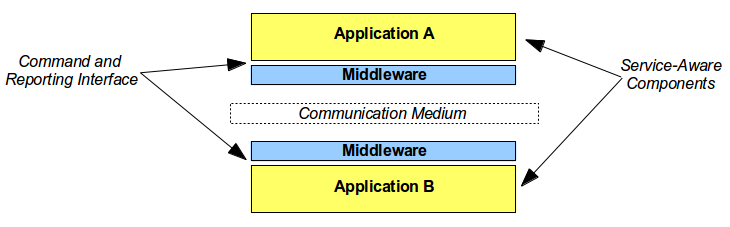
\includegraphics[scale=0.4,keepaspectratio=true]{Middleware.png}
 \caption{Applications and Middleware}
 \label{fig:Middleware}
\end{figure}
